\documentclass{article}

% if you need to pass options to natbib, use, e.g.:
%     \PassOptionsToPackage{numbers, compress}{natbib}
% before loading neurips_2025

% The authors should use one of these tracks.
% Before accepting by the NeurIPS conference, select one of the options below.
% 0. "default" for submission
 \usepackage{neurips_2025}
% the "default" option is equal to the "main" option, which is used for the Main Track with double-blind reviewing.
% 1. "main" option is used for the Main Track
%  \usepackage[main]{neurips_2025}
% 2. "position" option is used for the Position Paper Track
%  \usepackage[position]{neurips_2025}
% 3. "dandb" option is used for the Datasets & Benchmarks Track
 % \usepackage[dandb]{neurips_2025}
% 4. "creativeai" option is used for the Creative AI Track
%  \usepackage[creativeai]{neurips_2025}
% 5. "sglblindworkshop" option is used for the Workshop with single-blind reviewing
 % \usepackage[sglblindworkshop]{neurips_2025}
% 6. "dblblindworkshop" option is used for the Workshop with double-blind reviewing
%  \usepackage[dblblindworkshop]{neurips_2025}

% After being accepted, the authors should add "final" behind the track to compile a camera-ready version.
% 1. Main Track
 % \usepackage[main, final]{neurips_2025}
% 2. Position Paper Track
%  \usepackage[position, final]{neurips_2025}
% 3. Datasets & Benchmarks Track
 % \usepackage[dandb, final]{neurips_2025}
% 4. Creative AI Track
%  \usepackage[creativeai, final]{neurips_2025}
% 5. Workshop with single-blind reviewing
%  \usepackage[sglblindworkshop, final]{neurips_2025}
% 6. Workshop with double-blind reviewing
%  \usepackage[dblblindworkshop, final]{neurips_2025}
% Note. For the workshop paper template, both \title{} and \workshoptitle{} are required, with the former indicating the paper title shown in the title and the latter indicating the workshop title displayed in the footnote.
% For workshops (5., 6.), the authors should add the name of the workshop, "\workshoptitle" command is used to set the workshop title.
% \workshoptitle{WORKSHOP TITLE}

% "preprint" option is used for arXiv or other preprint submissions
 % \usepackage[preprint]{neurips_2025}

% to avoid loading the natbib package, add option nonatbib:
%    \usepackage[nonatbib]{neurips_2025}

\usepackage[utf8]{inputenc} % allow utf-8 input
\usepackage[T1]{fontenc}    % use 8-bit T1 fonts
\usepackage[vietnamese]{babel} % Thêm dòng này
\usepackage{hyperref}       % hyperlinks
\usepackage{url}            % simple URL typesetting
\usepackage{booktabs}       % professional-quality tables
\usepackage{amsfonts}       % blackboard math symbols
\usepackage{nicefrac}       % compact symbols for 1/2, etc.
\usepackage{microtype}      % microtypography
\usepackage{xcolor}         % colors

\usepackage{graphicx}
\usepackage{subcaption}
\usepackage{booktabs}
\usepackage{multirow}
\usepackage{array}
\usepackage{float}
\usepackage{xcolor}
\usepackage{amsmath}

% Note. For the workshop paper template, both \title{} and \workshoptitle{} are required, with the former indicating the paper title shown in the title and the latter indicating the workshop title displayed in the footnote. 
\title{DATATHON 2026 -- The Gridbreakers\\ Round 1: Breaking Business Boundaries\\ Nhóm: DanaScience
}


% The \author macro works with any number of authors. There are two commands
% used to separate the names and addresses of multiple authors: \And and \AND.
%
% Using \And between authors leaves it to LaTeX to determine where to break the
% lines. Using \AND forces a line break at that point. So, if LaTeX puts 3 of 4
% authors names on the first line, and the last on the second line, try using
% \AND instead of \And before the third author name.

\author{%
    \begin{tabular}{c c}
        Nguyễn Đăng Nhân$^1$ & Lê Tự Phong$^1$ \\
        Ngành Khoa học dữ liệu & Ngành Khoa học dữ liệu \\
        \texttt{dangnhan0610@gmail.com} & \texttt{phongletu78@gmail.com} \\[0.8em]
        Nguyễn Thành Bảo$^1$ & Đặng Thanh Huyền$^1$ \\
        Ngành Công nghệ thông tin & Ngành Khoa học dữ liệu \\
        \texttt{thanhbao0905@gmail.com} & \texttt{thanhhuyendang2006@gmail.com}
    \end{tabular}
    \AND
    {\small $^1$ Trường Đại học Khoa học tự nhiên, ĐHQG-HCM}
  % \And
  % Coauthor \\
  % Affiliation \\
  % Address \\
  % \texttt{email} \\
}

\definecolor{insightbox}{RGB}{232,248,240}
\definecolor{insightborder}{RGB}{45,106,79}
\definecolor{warnbox}{RGB}{255,243,205}
\definecolor{warnborder}{RGB}{230,76,51}

\newcommand{\insightbox}[1]{%
  \begin{center}
    \fcolorbox{insightborder}{insightbox}{%
      \begin{minipage}{0.93\linewidth}
        \small\textbf{$\rightarrow$ Insight:} #1
      \end{minipage}
    }
  \end{center}
}

\makeatletter
\@anonymousfalse
\makeatother


\begin{document}


\maketitle

\section{Tổng quan dữ liệu}
 
Bộ dữ liệu gồm 13 bảng mô phỏng hoạt động thương mại điện tử thời trang tại Việt Nam (2012--2022). Sau kiểm định chất lượng: không có bản ghi trùng lặp, nhất quán về khóa ngoại, các cột \texttt{null} hợp lệ theo đặc thù giao dịch (ví dụ \texttt{applicable\_category} trong \texttt{promotions}).
 
\section{Phần 2: Trực quan hóa và Phân tích Dữ liệu}
 
\subsection{Descriptive — Điều gì đã xảy ra?}
 
\begin{figure}[H]
  \centering
  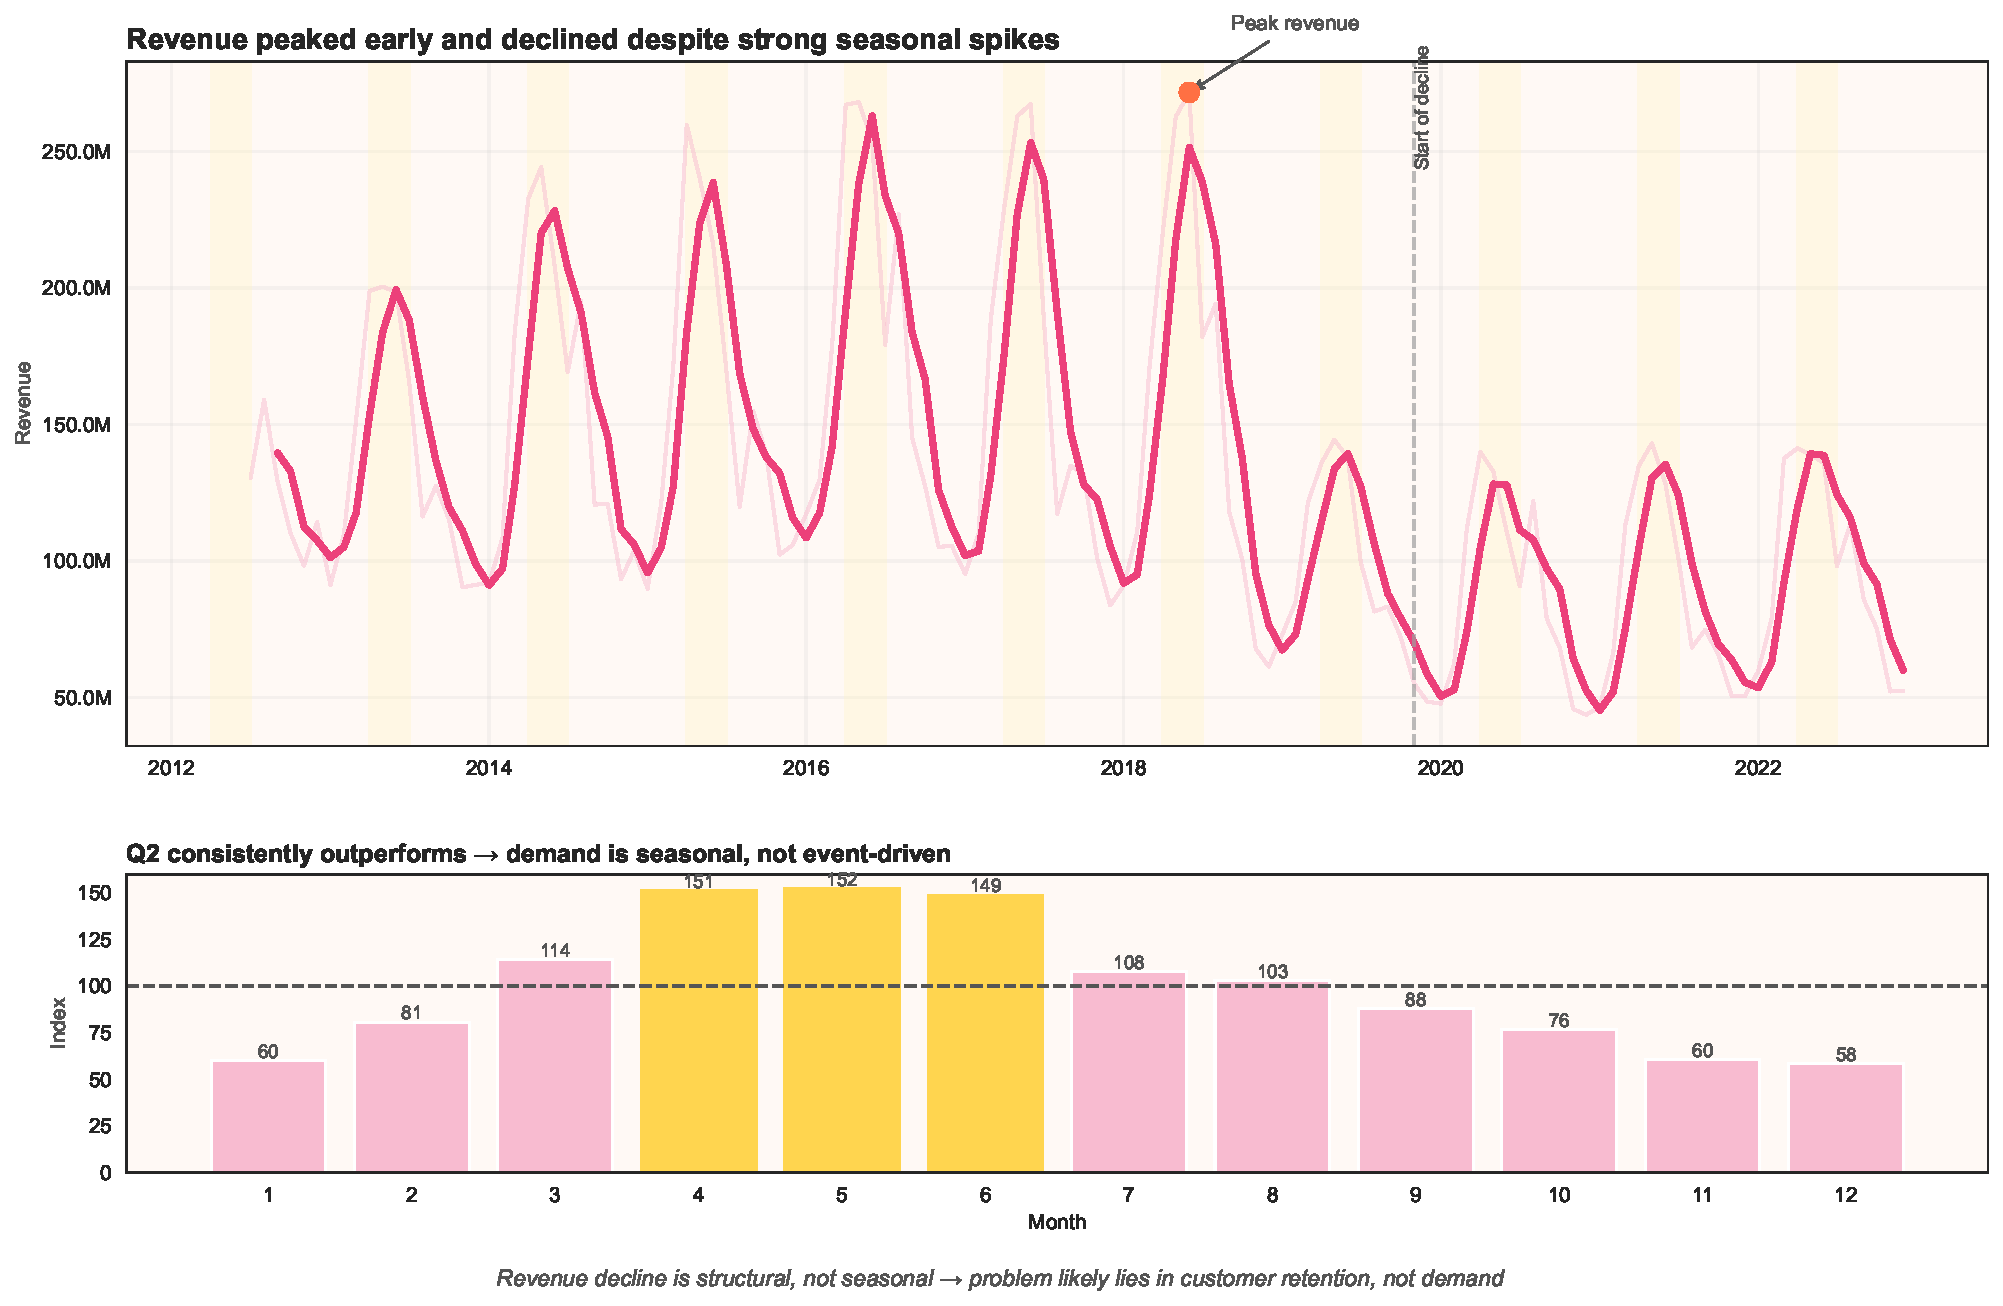
\includegraphics[width=0.72\textwidth]{../Part2/dataviz_chart1_descriptive.pdf}
  \caption{\textbf{Revenue Trend \& Seasonality Index (2012--2022).} Trên: doanh thu tháng và đường làm mịn 3 tháng; vùng vàng = Q2 cao điểm. Dưới: Seasonality Index (baseline = 100).}
  \label{fig:chart1}
\end{figure}
 
Doanh thu tăng đến đỉnh \textbf{2,10 tỷ VNĐ năm 2016} rồi giảm rõ từ 2019, ổn định ở mức 1,04--1,17 tỷ VNĐ giai đoạn 2020--2022. Cấu trúc mùa vụ vẫn nhất quán: Q2 luôn là đỉnh nhu cầu, tháng 5 đạt Seasonality Index \textbf{154} --- gấp 2,6× tháng 12. Dù Q2 năm nào cũng tạo đỉnh, giá trị đỉnh lại thấp dần qua từng năm --- khách hàng vẫn mua theo mùa, nhưng quy mô đang thu hẹp.
 
\insightbox{Vấn đề không nằm ở nhu cầu thị trường vì cấu trúc Q2 vẫn ổn định và dự báo được. Nguyên nhân sụt giảm nhiều khả năng đến từ việc doanh nghiệp \textbf{không giữ được khách hàng cũ} hoặc chưa bù đắp đủ lượng khách đã mất.}
 
\subsection{Diagnostic — Tại sao nó xảy ra?}
 
\begin{figure}[H]
  \centering
  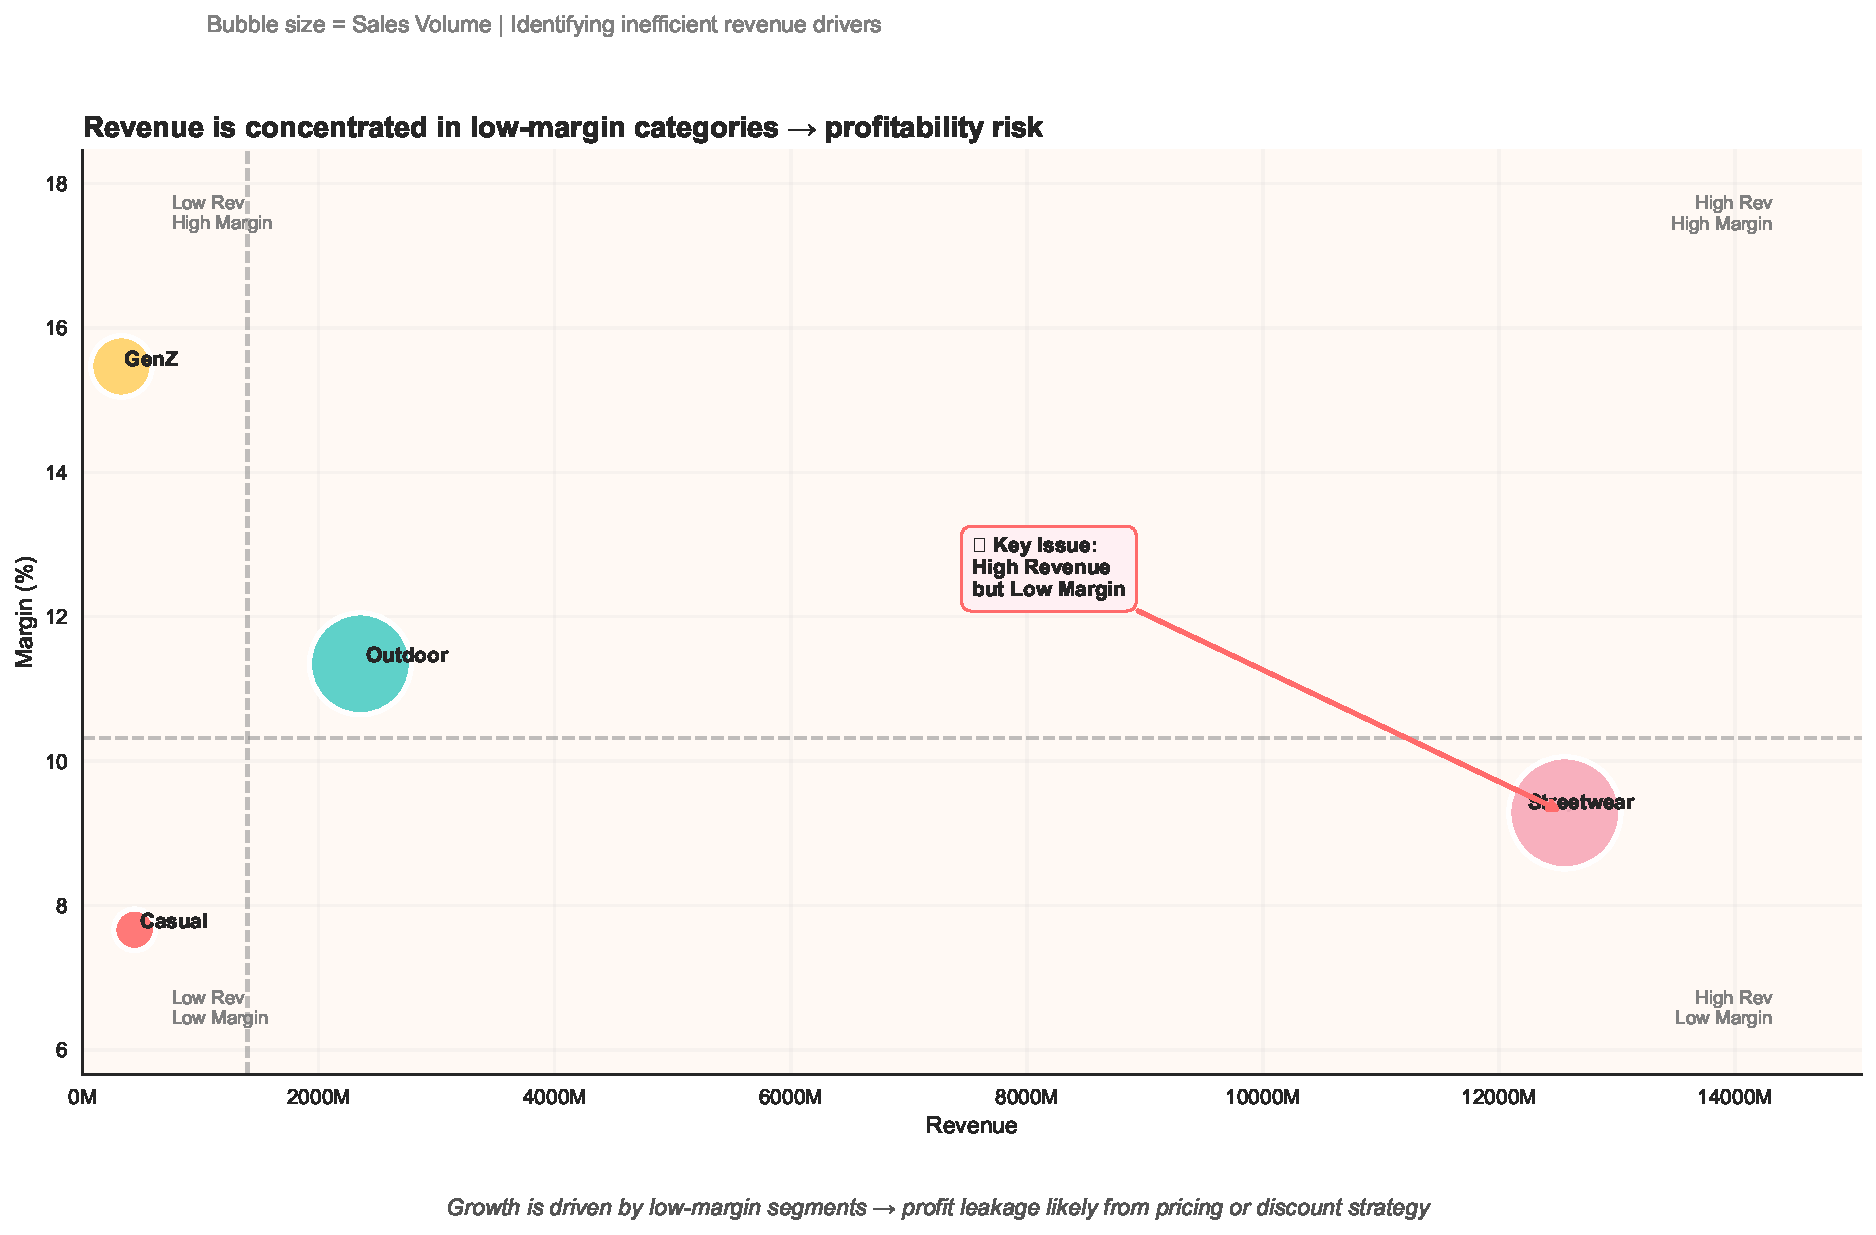
\includegraphics[width=0.72\textwidth]{../Part2/dataviz_chart2_diagnostic.pdf}
  \caption{\textbf{Revenue $\times$ Gross Margin Bubble Chart.} Kích thước bubble $\propto$ sản lượng bán. Panel phải: tỉ trọng Revenue vs. Profit theo danh mục.}
  \label{fig:chart2}
\end{figure}
 
\textbf{Streetwear} chiếm \textbf{79,9\% doanh thu} nhưng biên lợi nhuận thấp nhất (\textbf{13,2\%}), chỉ đóng góp \textbf{76,7\% lợi nhuận} --- đây là bẫy doanh thu điển hình: bán nhiều nhưng giữ lại ít. Ngược lại, \textbf{GenZ} có margin cao nhất (\textbf{19,1\%}) nhưng tỷ trọng chỉ 2,1\%, cho thấy dư địa rõ để dịch chuyển cơ cấu sản phẩm sang nhóm giá trị cao hơn.
 
\begin{figure}[H]
  \centering
  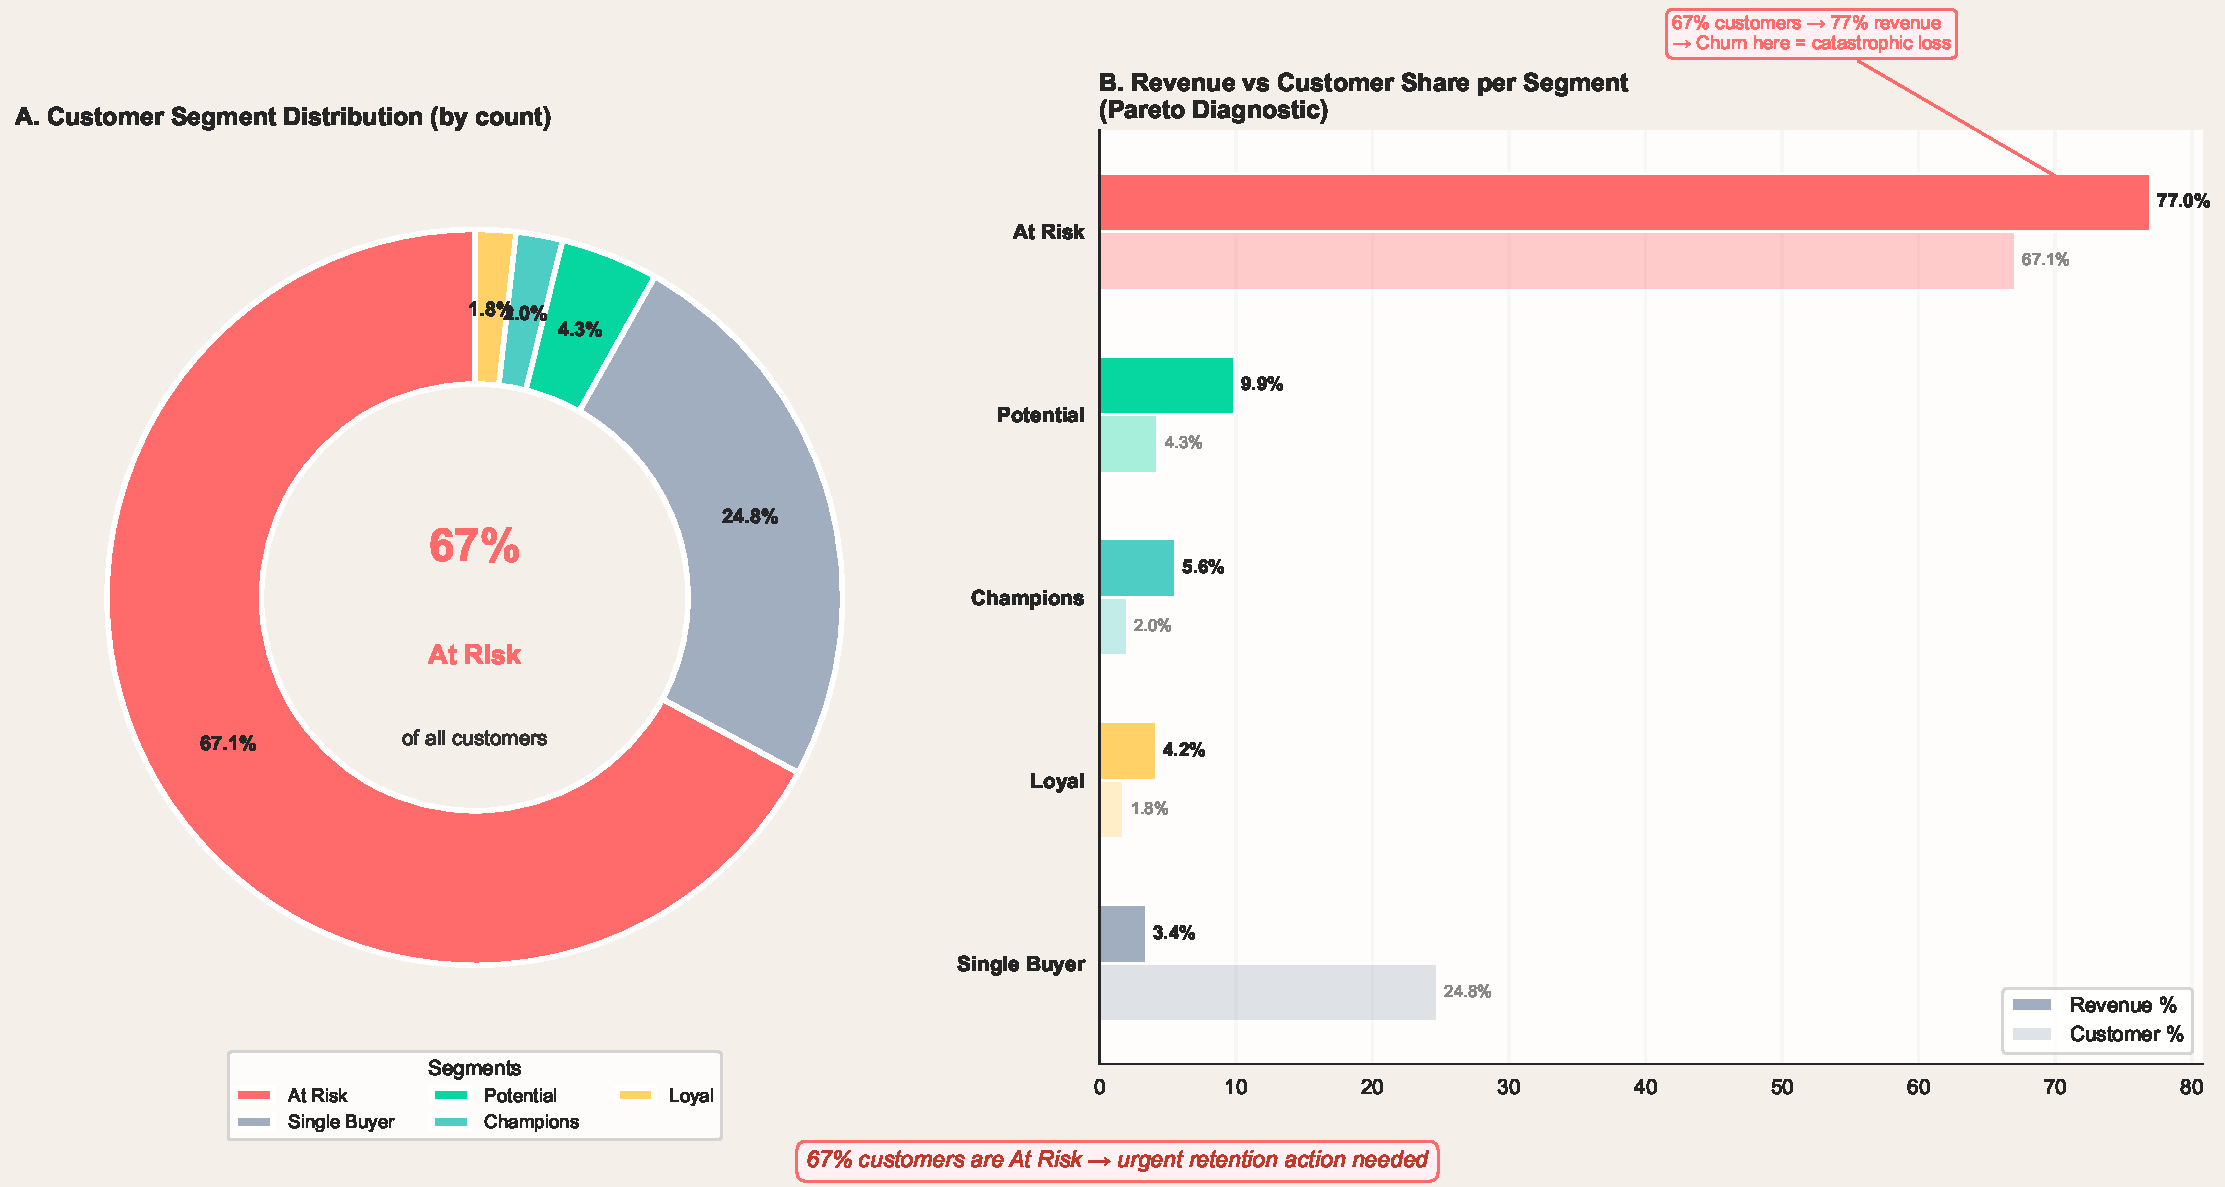
\includegraphics[width=0.72\textwidth]{../Part2/dataviz_chart3_diagnostic.pdf}
  \caption{\textbf{RFM Customer Health.} Trái: phân bổ khách hàng theo segment. Phải: \% Revenue vs. \% Customer theo segment.}
  \label{fig:chart3}
\end{figure}
 
Phân tích RFM cho thấy nhóm \textbf{At Risk} chiếm \textbf{67\%} khách hàng nhưng đóng góp tới \textbf{77\% doanh thu} --- rủi ro tập trung rất lớn. Khoảng \textbf{24,8\%} khách chỉ mua một lần rồi không quay lại, trong khi \textbf{Champions} và \textbf{Loyal} chỉ chiếm 3--4\%. Vấn đề cốt lõi không nằm ở thu hút khách mới mà ở năng lực giữ chân khách hiện có.
 
\insightbox{(1) Streetwear kéo biên lợi nhuận xuống dù dẫn đầu doanh thu; (2) 67\% khách hàng đang ``At Risk'' và kiểm soát 77\% doanh thu --- mất nhóm này là mất phần lớn doanh nghiệp.}
 
\subsection{Predictive --- Điều gì có thể xảy ra?}
 
\begin{figure}[H]
  \centering
  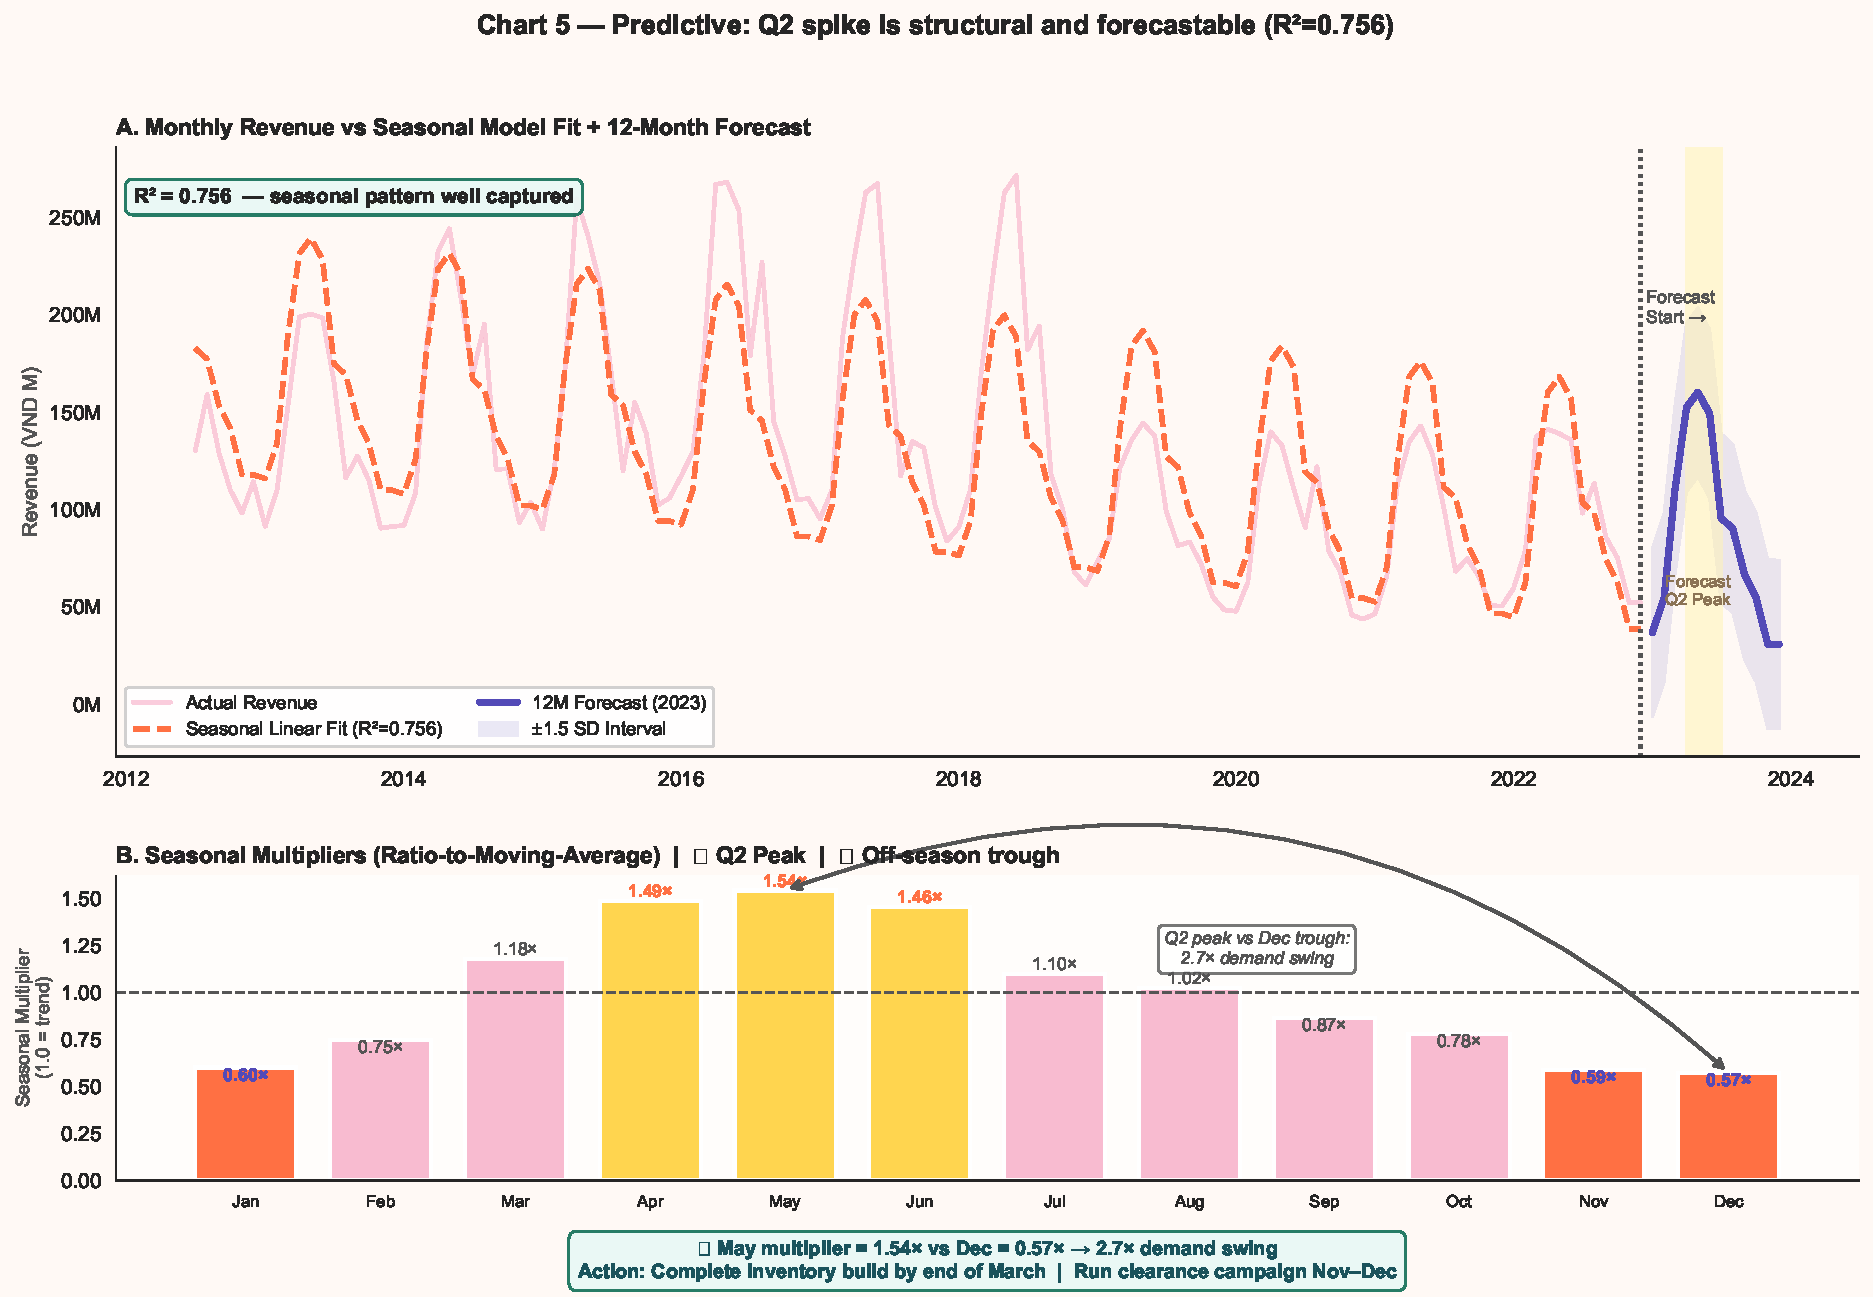
\includegraphics[width=0.72\textwidth]{../Part2/dataviz_chart5_predictive.pdf}
  \caption{\textbf{Trend Decomposition \& 12-Month Forecast.} Trên: doanh thu thực tế, model fit ($R^2{=}0{,}756$), dự báo $\pm1{,}5$~SD. Dưới: Seasonal multiplier; biên độ 2,7$\times$ giữa đỉnh T5 và đáy T12.}
  \label{fig:chart5}
\end{figure}
 
Mô hình hồi quy với seasonal dummies tháng đạt $R^2 = 0{,}756$, xác nhận pattern Q2 có thể dự báo với độ tin cậy cao. Tháng 5 đạt multiplier \textbf{1,54×}, tháng 12 chỉ còn \textbf{0,60×} --- biên độ \textbf{2,7×}. Đáng chú ý, xu hướng nền đang giảm nhẹ sau 2016: doanh nghiệp đang tăng trưởng nhờ ``cú hích'' mùa vụ hơn là nội lực bền vững.
 
\insightbox{Nhu cầu Q2 ổn định và dự báo được. Cần hoàn tất tích lũy tồn kho trước cuối tháng 3 để đón đỉnh T5; chạy clearance Nov--Dec khi multiplier ở mức thấp nhất (0,60×).}
 
\subsection{Prescriptive --- Chúng ta nên làm gì?}
 
\begin{figure}[H]
  \centering
  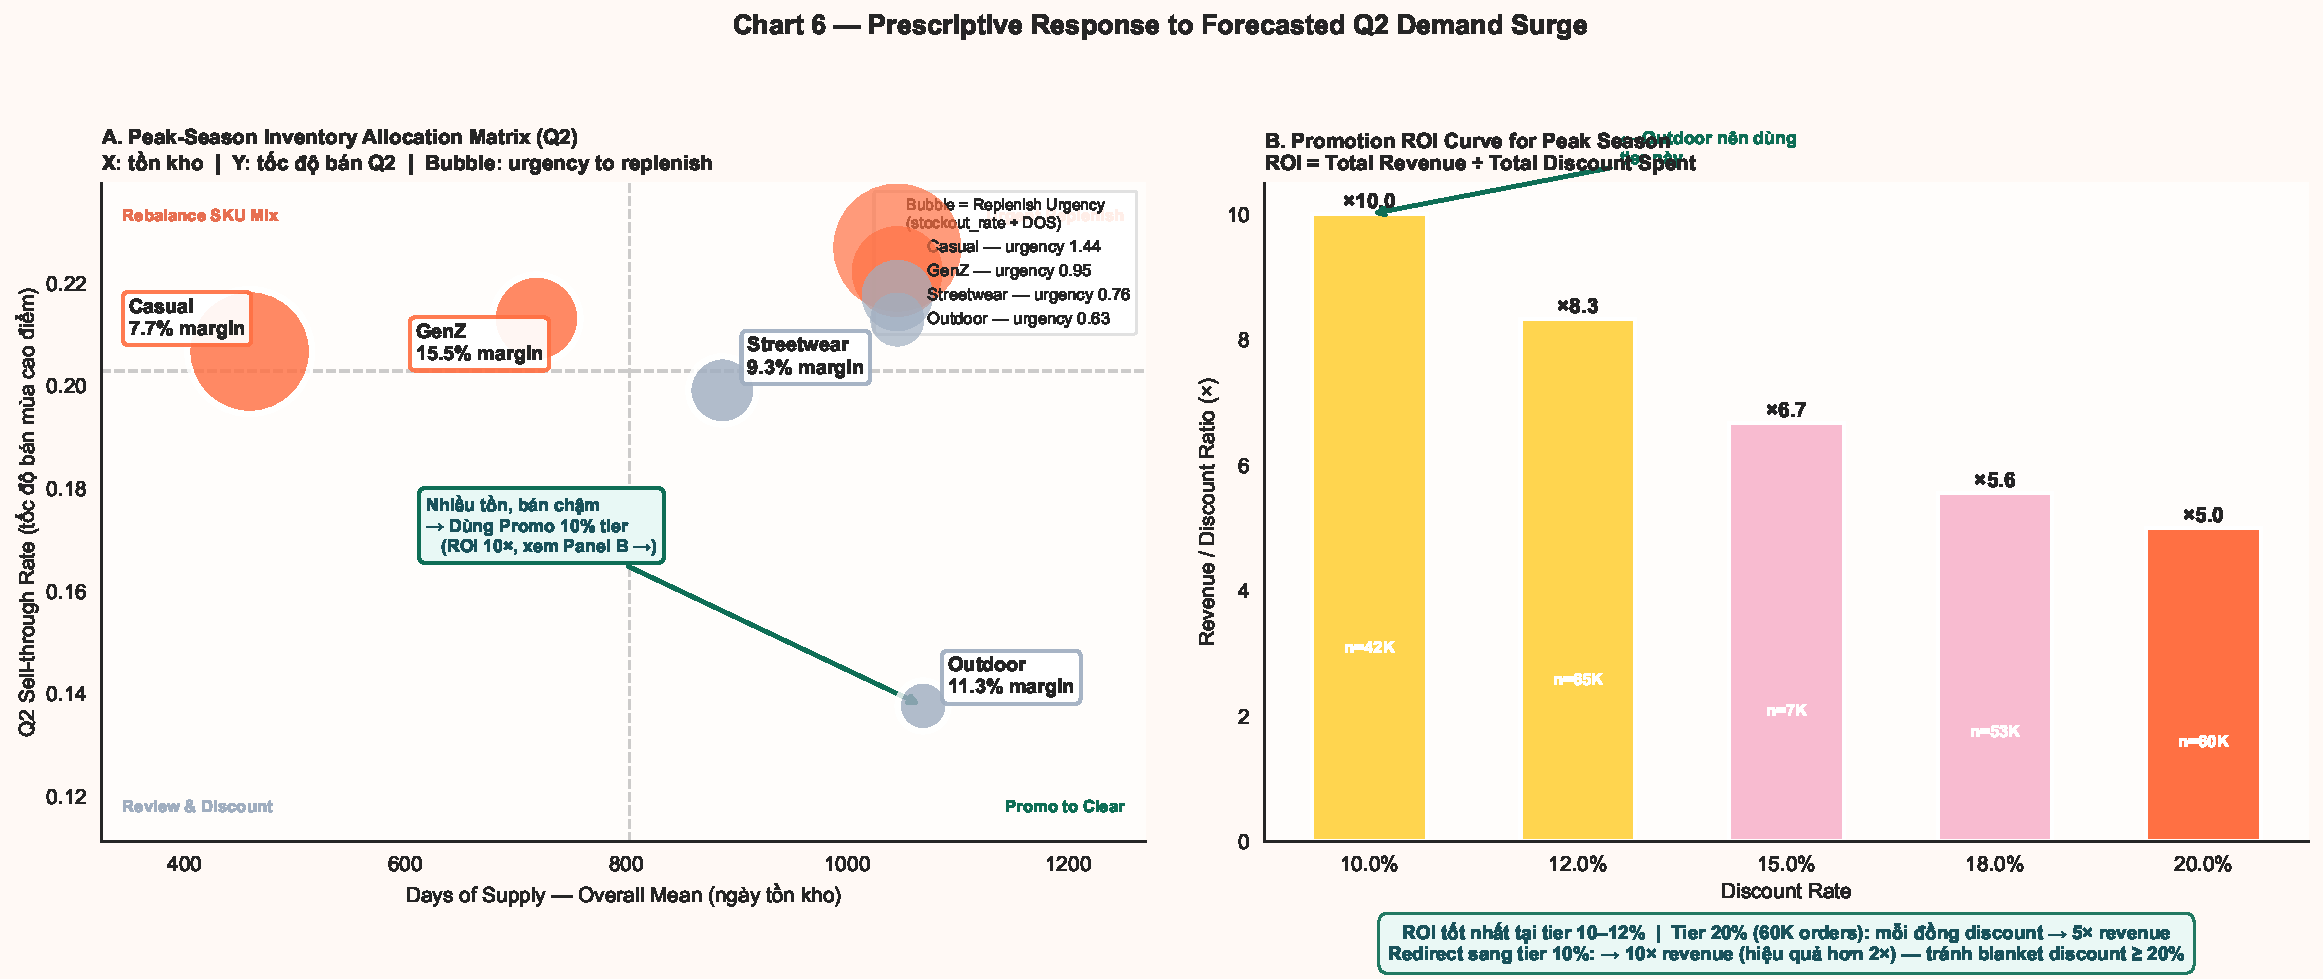
\includegraphics[width=0.72\textwidth]{../Part2/dataviz_chart6_prescriptive.pdf}
  \caption{\textbf{Inventory Allocation Matrix \& Promo ROI Curve.} Trái: DOS $\times$ Sell-Through Q2; bubble $\propto$ urgency score; nhãn = gross margin. Phải: ROI theo mức chiết khấu.}
  \label{fig:chart6}
\end{figure}
 
\textbf{Casual} có urgency score cao nhất (\textbf{1,44}) do DOS thấp và thường cháy hàng đúng cao điểm --- cần replenish ngay. \textbf{Outdoor} ở cực đối lập: DOS tới \textbf{1.069 ngày}, Sell-through Q2 chỉ \textbf{0,135} --- ứng viên rõ cho clearance promo. Curve ROI xác nhận điểm tối ưu chiết khấu tại \textbf{10\%} (ROI $\times$10,0), giảm còn $\times$5,0 khi tăng lên 20\% --- với 60.000 đơn đang dùng tier 20\%, đây là khoản lãng phí biên lợi nhuận có thể thu hồi ngay.
 
\insightbox{\textbf{Action plan Q2:} (1) Replenish Casual trước --- urgency cao nhất; (2) Promo 10\% cho Outdoor để giải phóng 1.069 ngày tồn kho, ROI $\times$10; (3) Giới hạn mọi discount $\leq 12\%$ --- vượt ngưỡng này ROI giảm một nửa dù doanh số tăng ngắn hạn.}

\section{Phần 3: Dự báo doanh thu}


\end{document}